\documentclass{beamer}
\usepackage[english,french]{layout}
\usepackage[utf8]{inputenc}
\usepackage[english]{babel}
\usepackage[T1]{fontenc}
\usepackage{lmodern}
\usepackage{textcomp}
\usepackage{amsmath, soul, color, multicol, type1cm, verbatim, latexsym, dsfont, float, listings,alltt}
\usepackage[official]{eurosym}
\usepackage{beamerthemesplit}
\usetheme{Frankfurt}
\usefonttheme{professionalfonts}
\setbeamercovered{transparent}
%NeSI Colors <-------------------------------------------------------------------------------------
\usecolortheme{lily}
\usecolortheme[RGB={47, 68, 71}]{structure} 
\definecolor{nesidark}{HTML}{2F4447}
\definecolor{nesilight}{HTML}{CED9DF}
\definecolor{nesigrey}{gray}{0.7}
\definecolor{nesilightgrey}{gray}{0.98}
\definecolor{nesidarkgrey}{gray}{0.3}
\definecolor{nesiblue}{HTML}{2B9FC2}
\setbeamercolor{block title}{fg=black,bg=nesigrey}
\setbeamercolor{block body}{bg=nesilightgrey,fg=nesidarkgrey}
\setbeamercolor{block body alerted}{bg=white,fg=black}
\setbeamercolor{alerted text}{bg=white,fg=black}
%NeSI Title <---------------------------------------------------------------------------------------
\setbeamerfont{title}{size=\huge}
\frenchspacing
\hyphenation{NeSI}
%NeSI Template parameters <-------------------------------------------------------------------------
\setbeamertemplate{blocks}[default]
\useinnertheme{circles}
\setbeamertemplate{title page}[default][center,rounded=false,shadow=false]
\newcommand\BackgroundPicture[1]{%
\setbeamertemplate{background}{%
\parbox[c][\paperheight]{\paperwidth}{%
\vfill \hfill \includegraphics[height=0.9\paperheight]{#1}
\hfill \vfill
}}}

%Content Starts Here <-------------------------------------------------------------------------------
\title{Rapid Parameterisation of Small Molecules}
%\subtitle{Computational Science team}
\author{Dr Benjamin Roberts \\ (ben.roberts@nesi.org.nz)}
\date{23 March 2015}

\begin{document}

{
\setbeamertemplate{background canvas}{
\includegraphics[height=0.99\paperheight]{NeSI_img/Slide00.png}} 
\begin{frame}[plain]
\vspace{1cm}
\titlepage
\end{frame}
}


% This will generate the outline. If you have several topics, uncomment the multicols 
\begin{frame}
\frametitle{Outline}
% \begin{multicols}{2} 
   \tableofcontents
% \end{multicols}
\end{frame}


%%%%%%%%%%%%%%%%%%%%%%%%%%%%%%%%%%%%%%%%%%%%%%%%%%%%%%%%%%%%%%%%%%%%%%%%%%%%%%%%%%%%%%%%%%%%%%%
%%%%%%%%%%%%%%%%%%%%%%%%%%%%%%%%%%%%%%%% Some Examples %%%%%%%%%%%%%%%%%%%%%%%%%%%%%%%%%%%%%%%%%%%
%%%%%%%%%%%%%%%%%%%%%%%%%%%%%%%%%%%%%%%%%%%%%%%%%%%%%%%%%%%%%%%%%%%%%%%%%%%%%%%%%%%%%%%%%%%%%%%

\section{The Background}
\subsection{Introduction to Molecular Mechanics}
\frame[t]
{
\frametitle{Molecular Mechanics}
\begin{itemize}
\item An approximation of a molecule's potential energy using a Newtonian model
\item Add a time component to get molecular dynamics (MD)
\item The system is represented in three parts: Coordinates, topology and force field
\item Coordinates: Where all the particles are (relative to each other)
\item Topology: Which particles are connected to which other particles
\item Force fields: What's the deal?
\end{itemize}
}
\subsection{Force Fields and Parameterisation}
\frame[t]
{
\frametitle{Force fields}
\begin{center}
{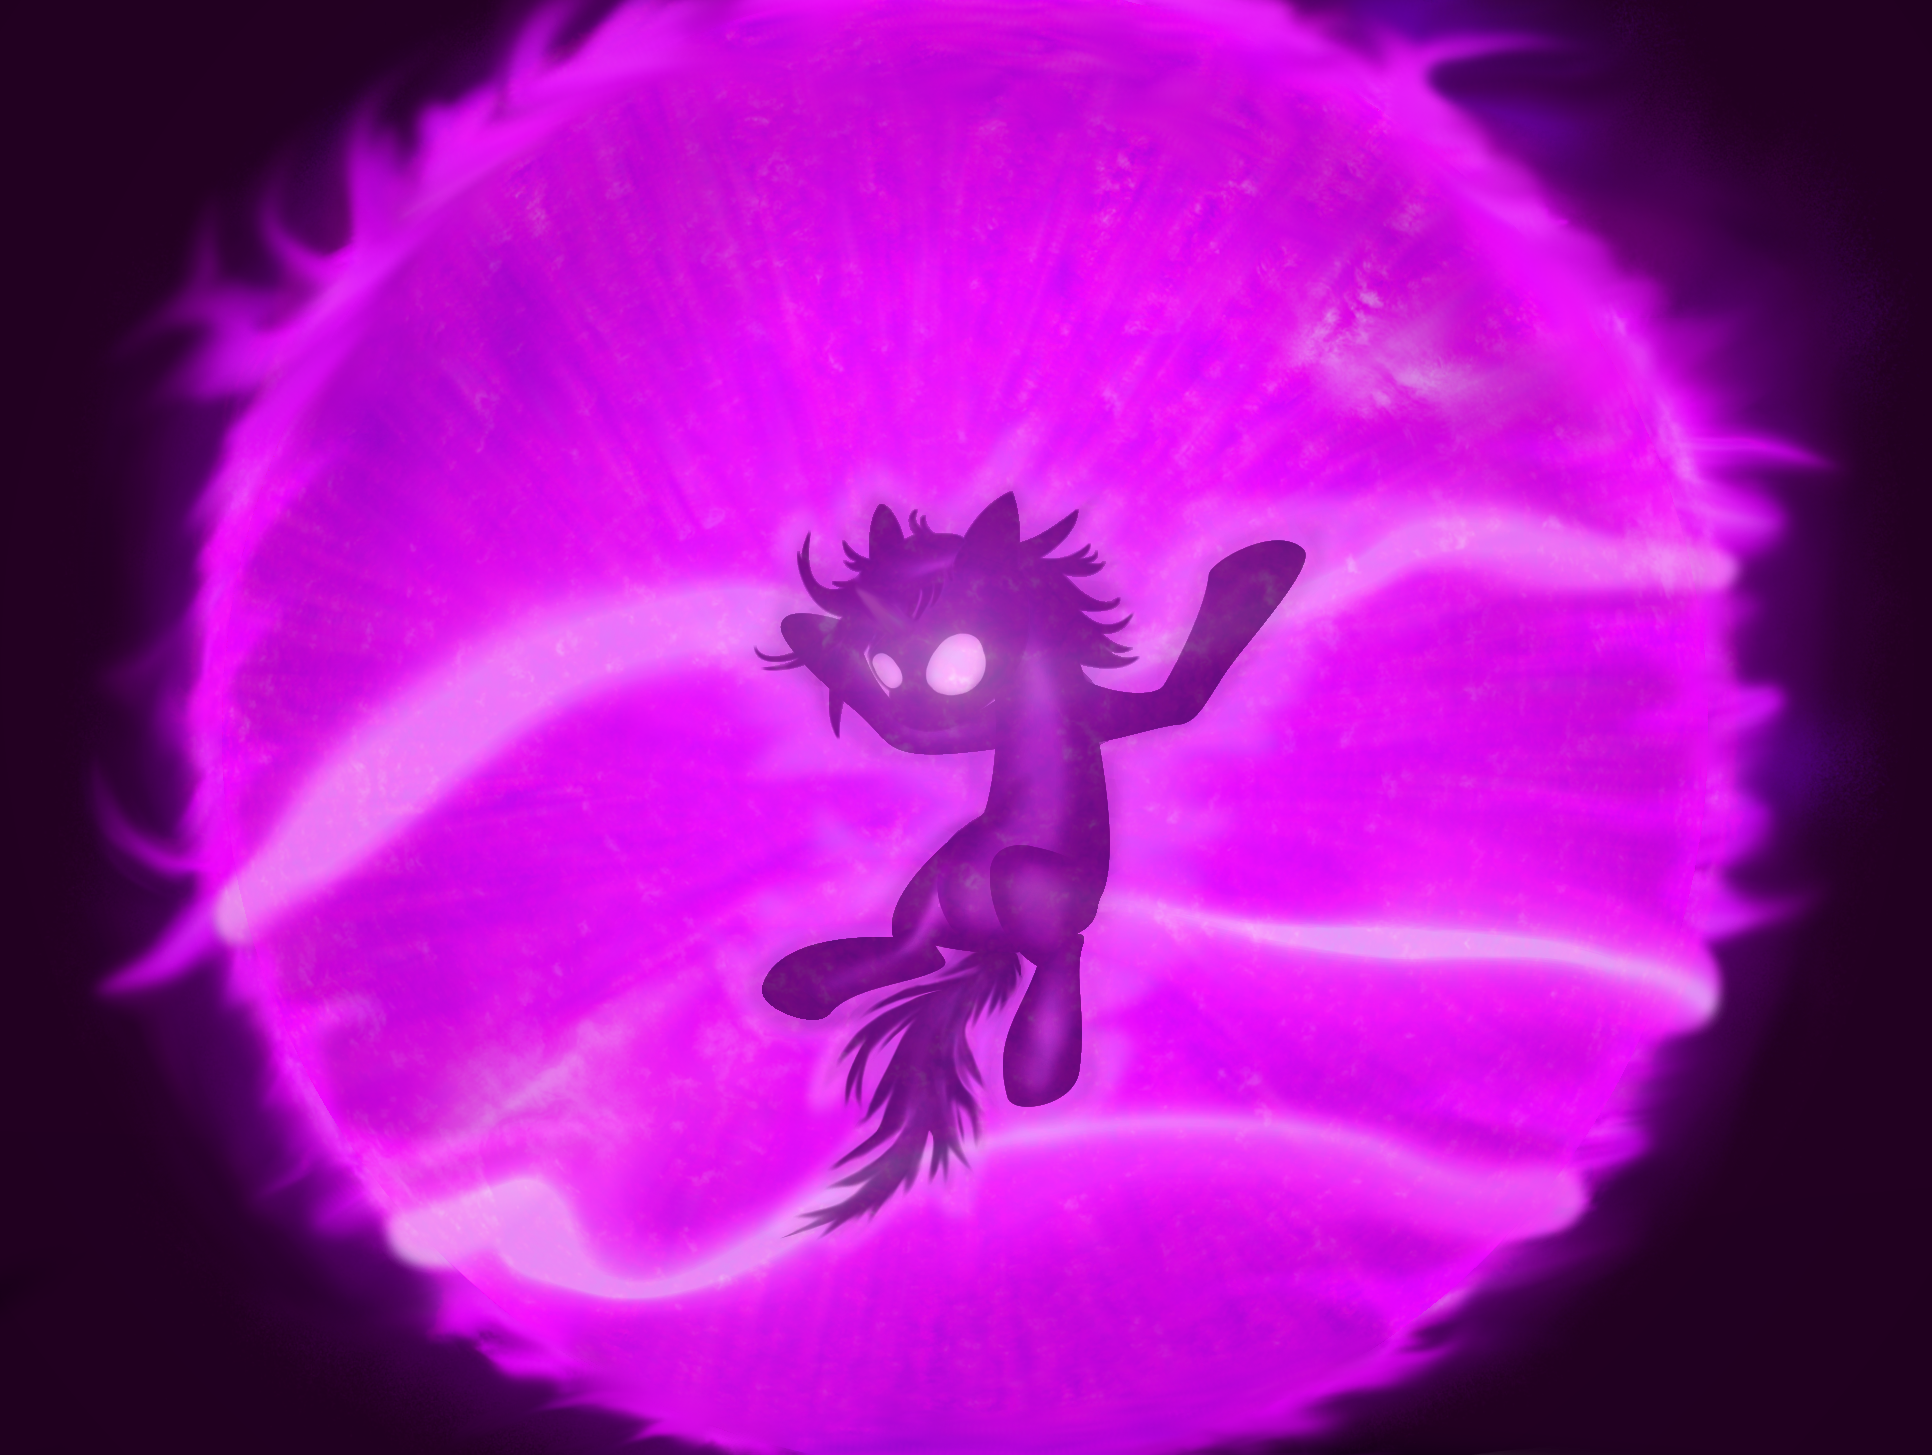
\includegraphics[height=0.45\paperheight]{force_field_by_konsumo-d78g7nt.png}}
\end{center}
A force field is an approximate mathematical model of the potential energy surface of the system.
It can be expressed as an equation in \(3N - 6\) variables, where \(N\) is the number of particles.
}
\frame[t]
{
\frametitle{Force fields}
\begin{block}{Functional form}
	\begin{itemize}
		\item The equations used to model interactions between particles
		\item All interactions of the same class will use the same basic model (e.g., bonds commonly use a quadratic equation in the manner of Hooke's law)
	\end{itemize}
\end{block}
\begin{block}{Parameters}
	\begin{itemize}
		\item The constant terms used in the equations
		\item Within any given class, each specific type of interaction will have its own parameters
		\item Individual interaction types are often quite fine-grained
	\end{itemize}
\end{block}
}

\section{The Challenge}

\frame[t]
{
\frametitle{The Case of the Missing Parameters}
\begin{block}{The Problem}
\begin{itemize}
\item The equation for the potential energy is a vast sum of terms
\item Each term makes use of at least one parameter (usually more than one)
\item If any parameter in any term is missing, the equation can't be solved!
\item Parameters don't exist for most molecules.
\end{itemize}
\end{block}
\begin{block}{The Solution}
	\begin{itemize}
		\item Parameterise on the fly...
		\item ...right?
	\end{itemize}
\end{block}
}

\frame[t]
{
\frametitle{The Case of the Missing Parameters}
{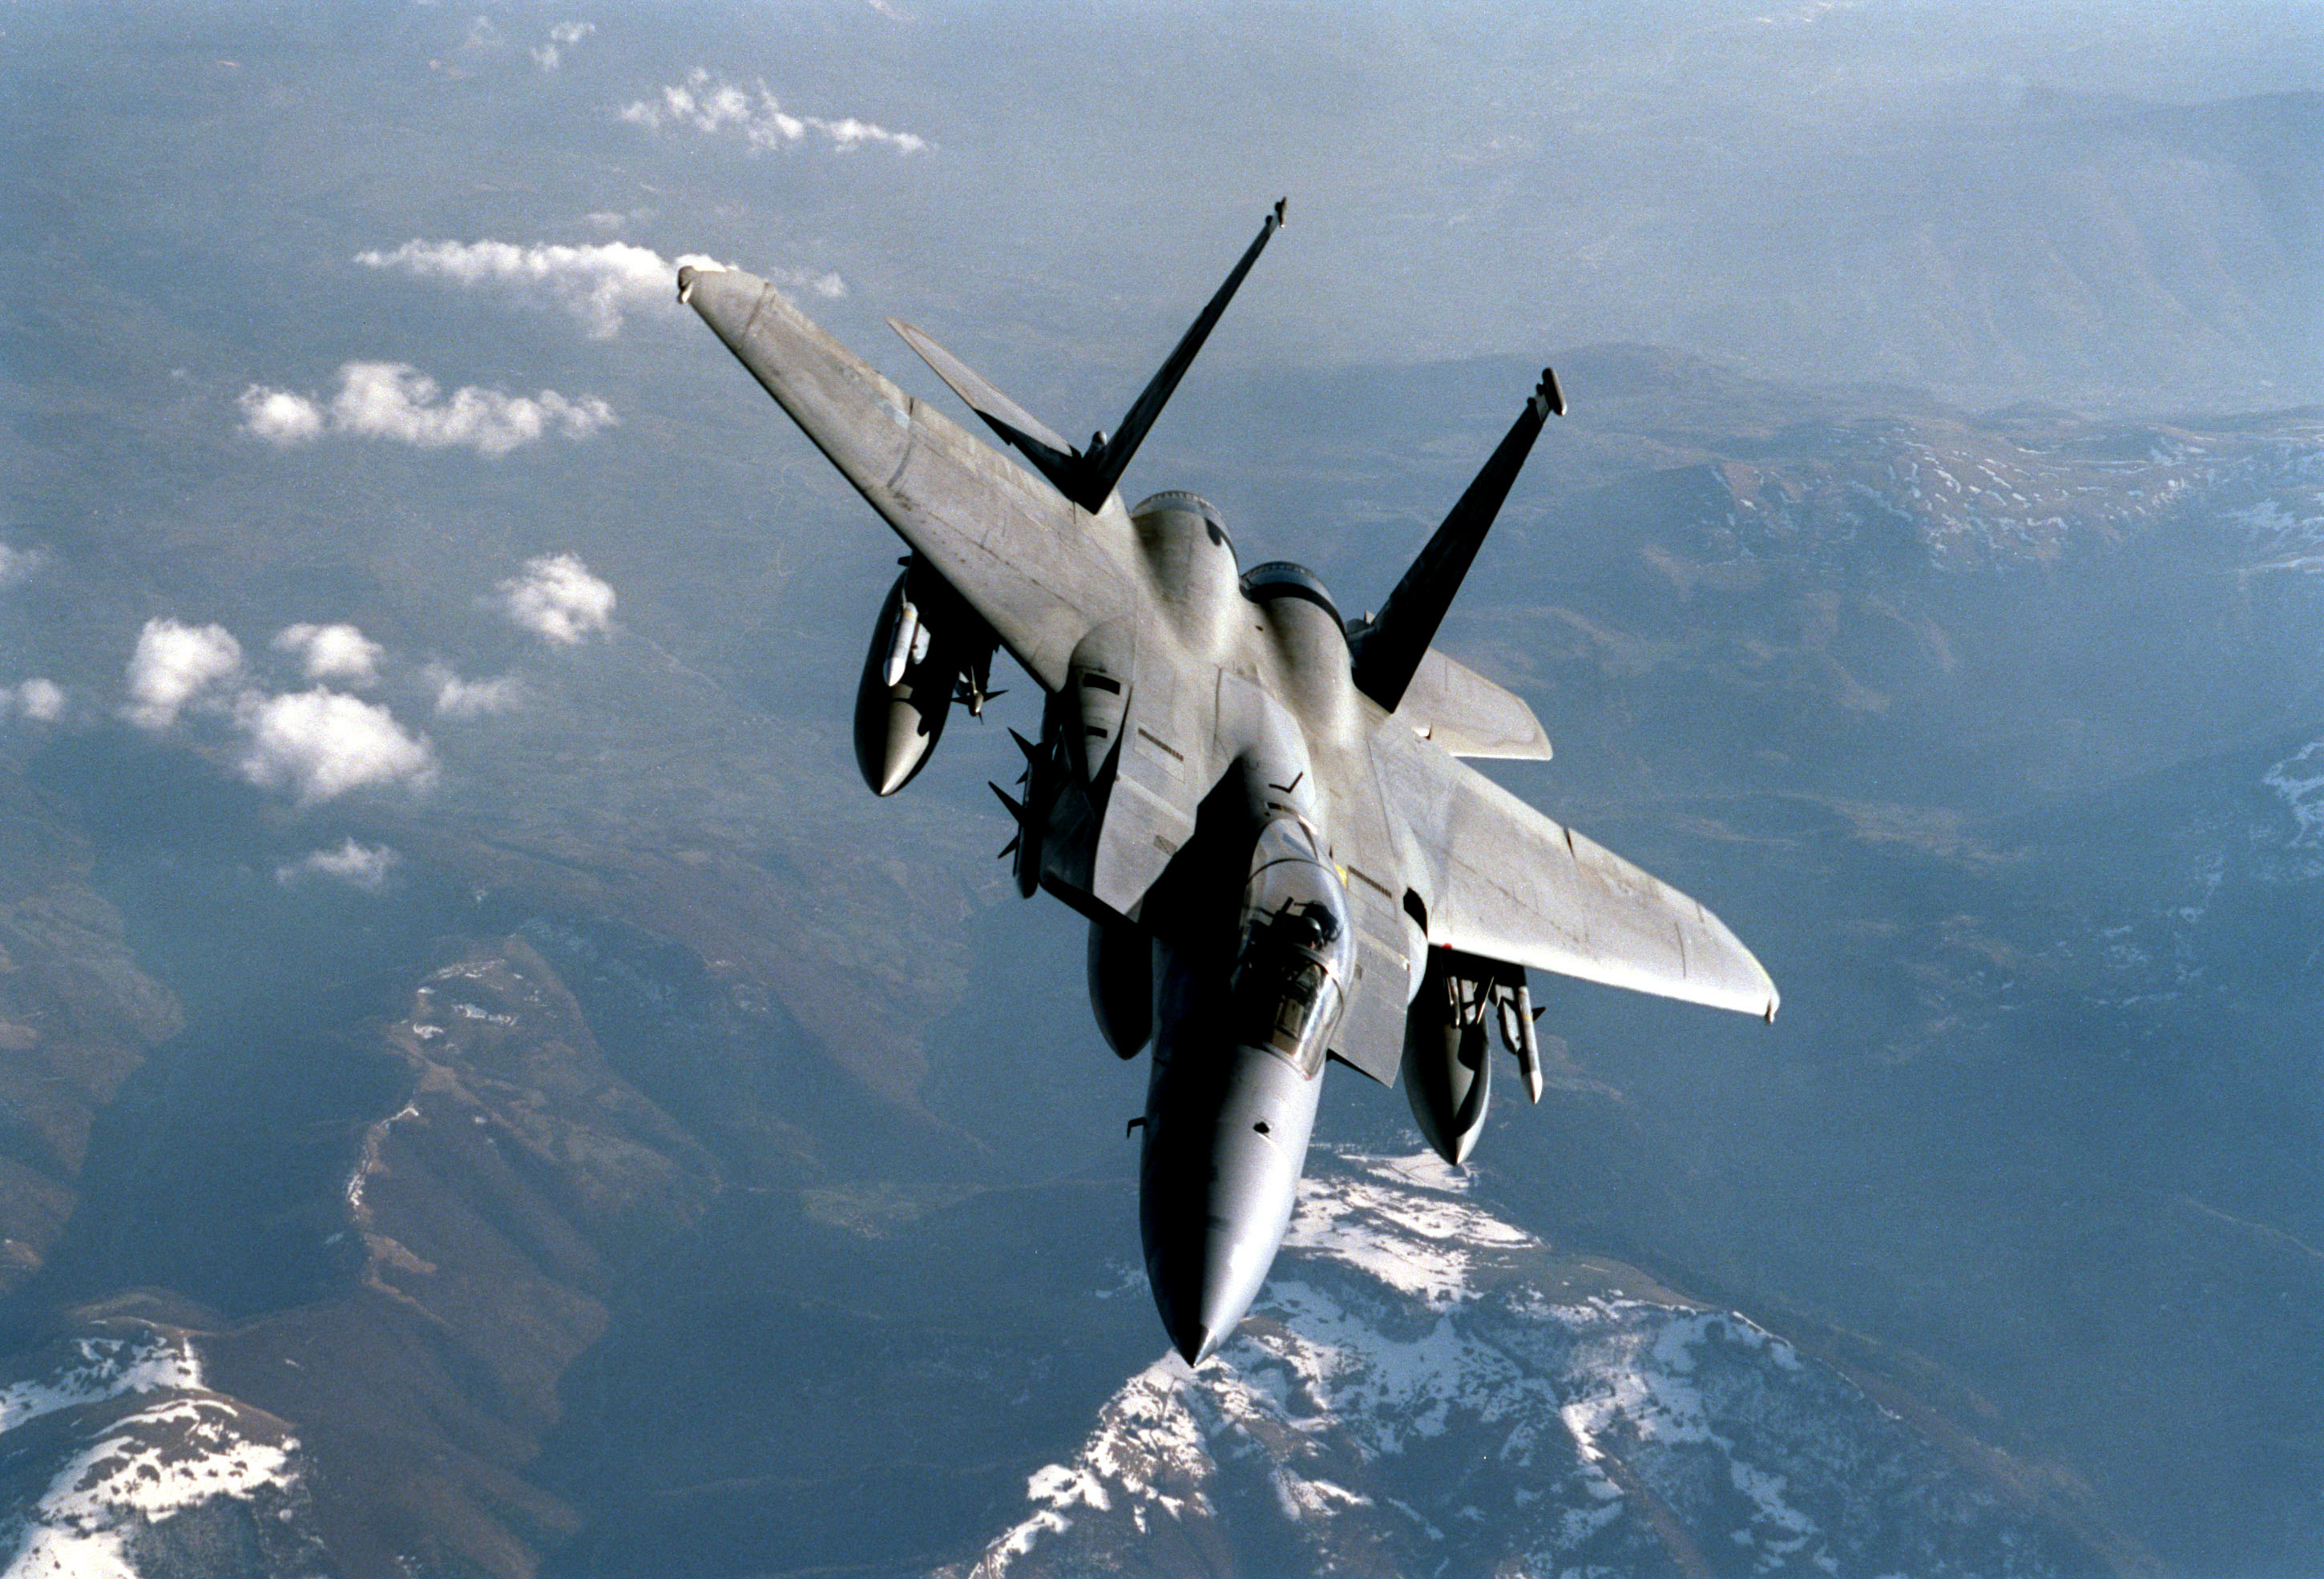
\includegraphics[height=0.3\paperheight]{F-15C.jpg}}
}

\frame[t]
{
\frametitle{The Case of the Missing Parameters}
{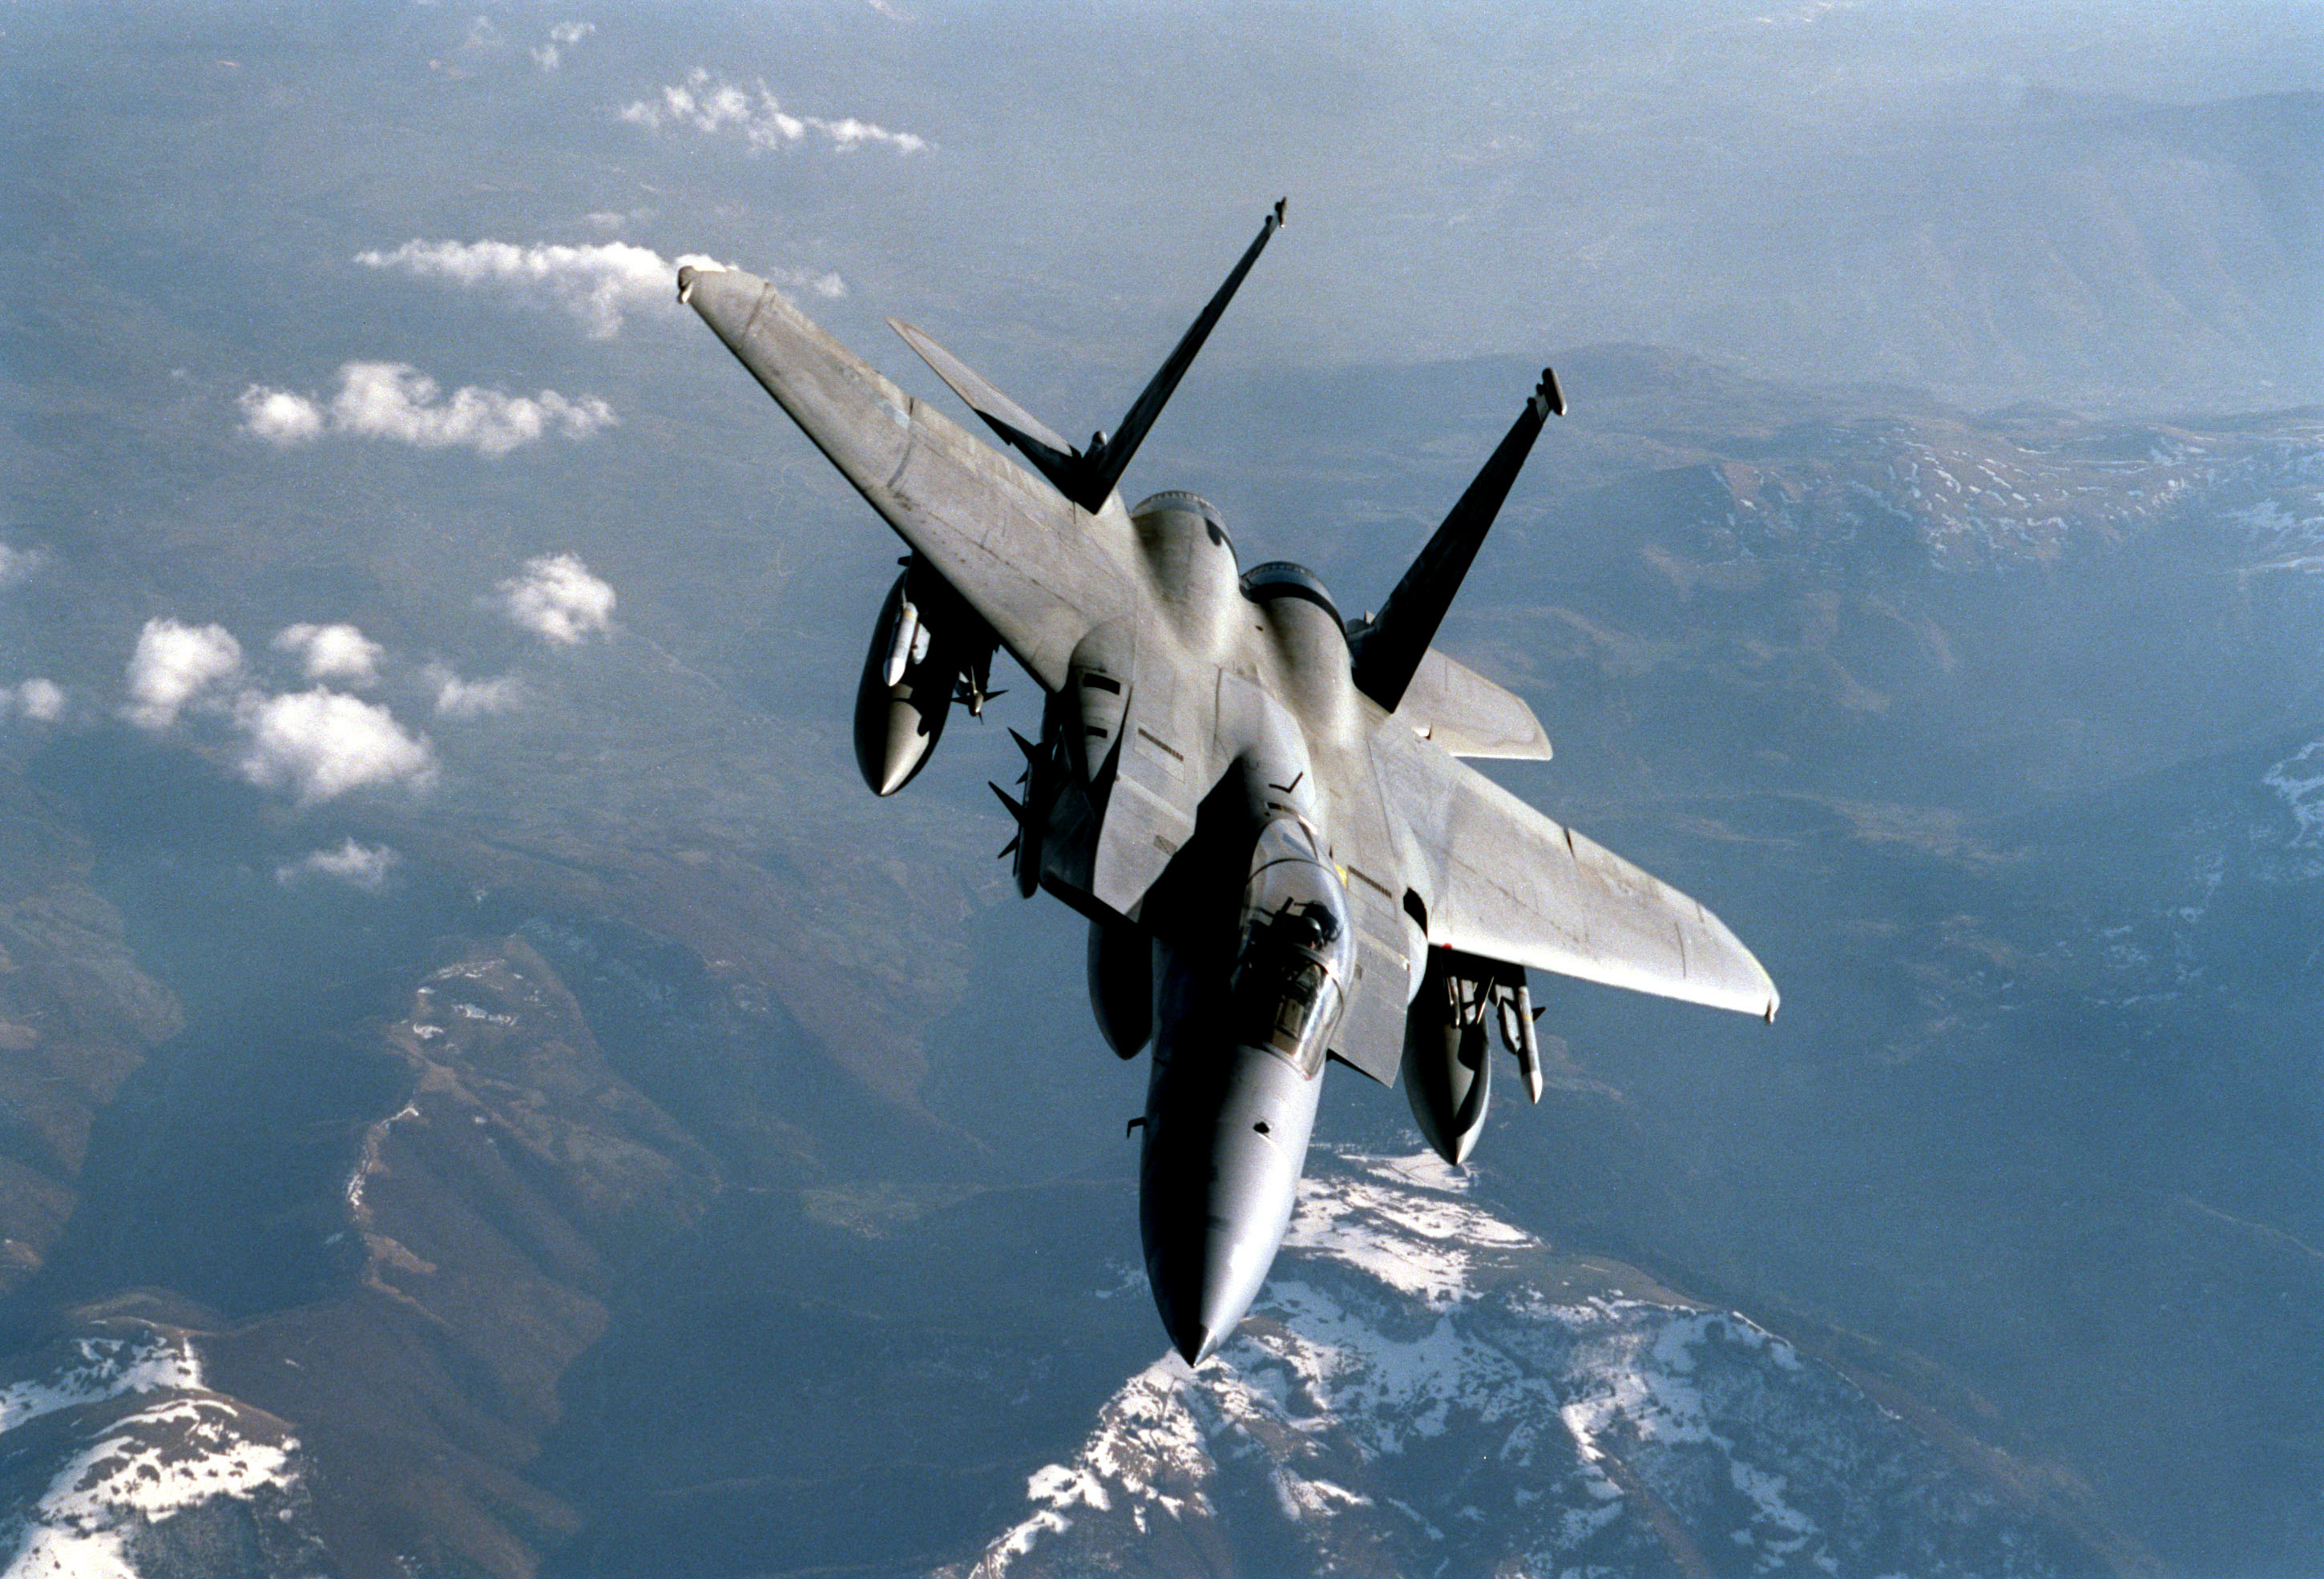
\includegraphics[height=0.3\paperheight]{F-15C.jpg}}
\linebreak
\begin{flushright}
{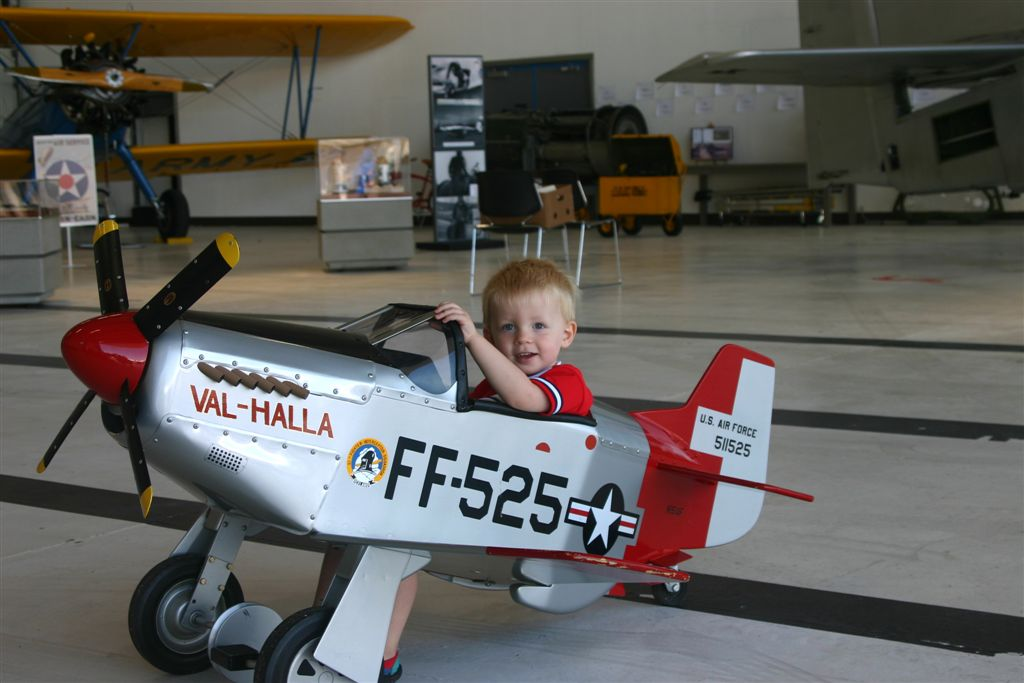
\includegraphics[height=0.3\paperheight]{bellingham.jpg}}
\end{flushright}
}

\section{How We're Tackling It}
\subsection{Overview}
\frame[t]
{
\frametitle{A Four-Step Approach}
 Our approach to parameter generation consists of four steps:
\begin{enumerate}
 \item Generate: Automated Topology Builder (ATB) http://compbio.biosci.uq.edu/atb/
 \item Refine: GAMESS-US quantum mechanical calculations
 \item Assemble: MAGIC
 \item Test: MD simulations
\end{enumerate}
}

\subsection{HPC-powered QM Refinement}
\frame[t]{
\frametitle{Refinement}
\begin{itemize}
	\item This is the slow part
	\item Up to 32 QM calculations per torsional degree of freedom
	\item The speed of each calculation depends on method and basis set
	\item Best if the calculations can be done in parallel
\end{itemize}
}

\frame[t]{
\frametitle{Workflow Development}
\begin{block}{Parallelisation}
	\begin{itemize}
		\item Within each calculation: Run GAMESS in parallel (MPI parallelisation)
		\item Between calculations: Run calculations for different torsional angles simultaneously
	\end{itemize}
\end{block}
\begin{block}{Hardware selection}
	\begin{itemize}
		\item Based on fitness for purpose (from benchmarking work)
		\item Goal: Fast, straightforward workflow
		\item AIX on POWER6 versus Red Hat on Intel: Tests run on Fitzroy (NIWA HPCF) and Pan (University of Auckland)
	\end{itemize}
\end{block}
}

\frame[t]{
\frametitle{Results So Far}
\begin{itemize}
	\item GAMESS works faster on Fitzroy than on Pan
	\item However, the GROMOS software (required by another part of the workflow) only compiles on Pan
	\item Preliminary results suggest Pan is the best facility for this work
	\item Workflow is still being developed but should facilitate rapid parameterisation of novel molecules
	\item NeSI CST members are available for consultation regarding machine selection for your workflow
\end{itemize}
}
\section {Wrap-Up}
\frame[t]{
\frametitle{Acknowledgements}
\begin{itemize}
	\item Jane Allison
	\item Ivan Welsh
	\item Fran\c{c}ois Bissey
	\item Fabrice Cantos
\end{itemize}
}

{
\setbeamertemplate{background canvas}{
\includegraphics[height=0.99\paperheight]{NeSI_img/Slide00.png}} 
\begin{frame}[plain]
\begin{center}
{\Huge Questions \& Answers}
\end{center}
\end{frame}
}

\end{document} 
